\chapter{Communication between devices}
Key words: Master slave, block diagram, pull up res, cmd controlled,  
pi pull up = $1.8k\Omega$
\section{I$^2$C}

The I$^2$C (Inter-Integrated Circuit) protocol is a very used in electronic devices. It is a two way communications protocol 


\begin{figure}[!ht]
	\centering
	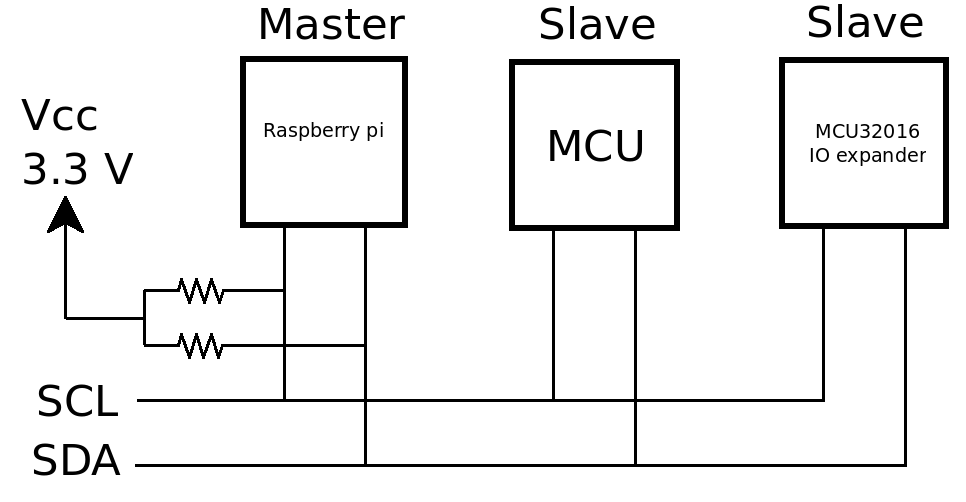
\includegraphics[width=0.8\textwidth]{communication_i2c_diagram.png}
	\caption{Block diagram of the I$^2$C bus}
	\label{fig:communication_I2C_diagram}
\end{figure}

\section{Implementation}

\subsection{I$^2$C Commands}
\begin{itemize}
	\begin{item}
		\textbf{ CMD 0x05}: cmd set led
	\end{item}

	\begin{item}
		\textbf{ CMD 0x10}: cmd get speed
	\end{item}
	
	\begin{item}
		\textbf{ CMD 0x20}: cmd set speed
	\end{item}	
	
	\begin{item}
		\textbf{ CMD 0x30}: cmd set dir
	\end{item}

	\begin{item}
		\textbf{CMD 0x50}: cmd set state
	\end{item}
	
	\begin{item}
		\textbf{ CMD 0x60}: cmd set target pos
	\end{item}
	
	\begin{item}
		\textbf{CMD 0x70}:  cmd precision stop
	\end{item}

	\begin{item}
		\textbf{CMD 0x80 }: cmd get dist
	\end{item}
	
	\begin{item}
		\textbf{CMD 0x90 }: cmd enable dist
	\end{item}			

	\begin{item}
		\textbf{ CMD 0xA0}: cmd is stable
	\end{item}		

\end{itemize}